% Define the module top matter
% This gets used to create the chapter title page
% NOTES:
%  * When multiple people have authored or contributed to the module, simply use a LaTeX line break
%    (a double-backslash: \\) at the end of each person.
%  * If you don't want this information shown on the module chapter page, simply remove the lines
%    within the \setModuleAuthors{} and \setModuleContributions{} environments
\setModuleTitle{Introduction to Snakemake}
\setModuleAuthors{%
  Nathan S. Watson-Haigh \mailto{nathan.watson-haigh@adelaide.edu.au}
}
%\setModuleContributions{%
%  John Doe \mailto{john.dow@example.com}%
%}

% BEGIN: Module Title Page
% This simply uses the above information and creates a module chapter page
% NOTES:
%  * The chapter page will always appear on odd numbered page
\chapter{\moduleTitle}
\newpage
% END: Module Title Page


% BEGIN: KLOs
% Key Learning Outcomes (KLOs) are an important aspect of any learning/training. They provide
% valuable infomation about what the trainee will have learned, what they will be able to do or know
% abouti at the end of the module. Unlike objectives which are more trainer oriented, KOLs are
% focused on the learner.
% At the end of the module, the KLOs can be used to develop criteria for writing an assessment to
% see if the trainees knowledge/skills have improved as a result of the module.
% 
% Search online for information on how to write KLOs. e.g.
% http://www.teaching-learning.utas.edu.au/__data/assets/word_doc/0014/23333/Learning-outcomes-v9.1.doc
\section{Key Learning Outcomes}

After completing this module the trainee should be able to:
\begin{itemize}
  \item Install Snakemake in a conda environment
  \item Execute a Snakemake workflow
  \item Use the provided ``profile'' to execute jobs on a compute cluster
  \item Write simple Snakemake rules capable of generating some output(s) by executing some code which perates on some input(s)
\end{itemize}
% END KLOs

% BEGIN: Resources Used
% This section can be used to describe the tools and data used during the module. It helps to act as
% a future reference to the trainee
\section{Resources Required}

For the purpose of this training you need access to:

\begin{itemize}
  \item A compute cluster with the \texttt{module} command available to you for loading software
  \item Singularity (\url{https://sylabs.io/singularity/}) - available as a module on the above cluster
  \item Conda(\url{https://www.anaconda.com/distribution/}) - available as a module on the above cluster
\end{itemize}


\subsection{Tools Used}
\begin{description}[style=multiline,labelindent=0cm,align=left,leftmargin=0.5cm]
  \item[Snakemake]\hfill\\
    \url{https://snakemake.readthedocs.io}
  \item[Graphviz]\hfill\\
    \url{https://www.graphviz.org}
\end{description}

\section{Useful Links}
 
\begin{description}[style=multiline,labelindent=0cm,align=left,leftmargin=0.5cm]
  \item[Slurm Documentation]\hfill\\
    \url{https://slurm.schedmd.com/documentation.html}
\end{description}

\newpage
% END: Resources Used

%========================
\section{Setting Up Your Environment}
%========================

For the purpose of the workshop we will be working on the head node of an HPC cluster running slurm (\url{https://slurm.schedmd.com/documentation.html}).
This is the most likely infrastructure that fellow bioinformaticians already find themselves using
on a regular basis. We also assume that the cluster provides the \texttt{module} command for you to
load software and the modules \texttt{Anaconda3} and \texttt{Singularity} are available to use.

The execution of the Snakemake workflow will actually take place on the cluster head node with jobs
being submitted to Slurm for queing and processing. From the head node, Snakemake will monitor the
submitted jobs for their completion status and submit new jobs as dependent jobs complete sucessfully.

%------------------------
\subsection{Connect to the Cluster Head Node}
%------------------------

\begin{steps}
First up, lets connect to the head node of the HPC cluster using \texttt{ssh}.

\emph{See your local facilitator for connection details. You should have one user account per person.}
\end{steps}

%------------------------
\subsection{Install Snakemake}
%------------------------

The recommended installation route for Snakemake is through a conda environemnt
(\url{https://snakemake.readthedocs.io/en/stable/getting_started/installation.html}). As such, you need
Anaconda3, usually avaiable to you on your cluster via the module system.

\begin{steps}
\begin{lstlisting}
# We use a specific version for reproducibility reasons
# Find the latest version: https://anaconda.org/search?q=snakemake
SNAKEMAKE_VERSION="5.5.4"

# Load miniconda
module load \
  miniconda3-4.6.14-gcc-5.4.0-kkzv7zk

#####
# One-time commands to integrate conda into bash
#####
conda init bash
. ~/.bashrc
#####

# Install snakemake by submitting a job to slurm - conda is a resource
# hog so your HPC sysadmins will like you for doing this
# This might take 10-20mins
sbatch --job-name 'snakemake-install' --mem 4G --time 30:00 --wrap \
 "conda create \
  --name snakemake \
  --channel bioconda --channel conda-forge \
  --yes \
  snakemake=${SNAKEMAKE_VERSION}"
\end{lstlisting}

The above \texttt{conda create} command, submitted to slurm, will take 10-20mins to complete. 

\end{steps}

\begin{note}

You can monitor all jobs in the slurm squeue, or just your own job(s) using the slurm command \texttt{squeue}:

\begin{lstlisting}
# All jobs in the queue
squeue

# Just your own jobs
squeue --user ${USER}
\end{lstlisting}

For convienience we have provided you with the \texttt{sq} function which produces nicer output than the default \texttt{squeue} and only shows your own jobs:

\begin{lstlisting}
# Your own jobs
sq

# Someone elses jobs
sq --user ${SOMEONE_ELSE}
\end{lstlisting}

\end{note}

Once your job completes successfully, snakemake installation is complete. All that is left to do is to
activate the environment which will make \texttt{snakemake} available on the command line:

\begin{steps}

\begin{lstlisting}
# Activate the newly created conda environment
conda activate snakemake
\end{lstlisting}

Integrate Snakemake autocompletion into bash:

\begin{lstlisting}
complete -o bashdefault -C snakemake-bash-completion snakemake
\end{lstlisting}

Test if Snakemake is actually working:

\begin{lstlisting}
snakemake --version
\end{lstlisting}

\end{steps}

If you experience problems with the installation, head to the \hyperref[sec:snake_trouble]{Troubleshooting} section for help.

\begin{bonus}
While waiting for others to catch up, why not have a look into how you would go about updating \texttt{Snakemake}
within this conda environment if there is a new version available.

\begin{answer}
\begin{lstlisting}
conda update \
  --channel bioconda --channel conda-forge \
  snakemake
\end{lstlisting}
\end{answer}

\end{bonus}


%========================
\section{Snakemake basics}
%========================

The way Snakemake runs can be thought of as being somewhat like a satellite navigation system, you request a destination
(``target'') and the system works out a route to get you there using its knowledge of the roads (``dependancies'') which
link together towns (``files'').

To exemplify the basics of Snakemake, we're going to take a look at constructing a ``Hello, world!'' example. We will go
through the process of explicitly defining ``rules'', the basic building blocks of a Snakemake workflow. Rules are used to
define how to create output (``target'') files, possibly requiring some \texttt{input} files. We will then work to
generalise these rule, introducing other Snakemake concepts and features along the way.

%------------------------
\subsection{Rule Definition}
%------------------------

By convention, we use a file called \texttt{Snakefile} in which to define our workflow rules. ``Rules'' define how to
create output (target) files. For example:

\begin{lstlisting}
rule hello_world:
	output:
		"Hello/World.txt",
	shell:
		"""
		echo "Hello, World!" > Hello/World.txt
		"""
\end{lstlisting}

This rule has the name \texttt{hello\_world} (line 1). The \texttt{output} file (line 3) is created by a \texttt{shell} script (line 6) which is
simply echoing a string, \texttt{Hello, world!}, and redirecting that into the appropriately named output file.

\begin{steps}

Create a working directory under \texttt{/shared/\$\{USER\}}, and add the above \texttt{hello\_world} rule to a file called \texttt{Snakefile}:

\begin{lstlisting}
# Create a working directory and move into it
mkdir -p /shared/${USER}/my_hello_world
cd /shared/${USER}/my_hello_world

# Create the Snakefile with the relevant contents using this heredoc
cat >Snakefile <<EOF
rule hello_world:
  output:
    "Hello/World.txt",
  shell:
    """
    echo "Hello, World!" > Hello/World.txt
    """
EOF
\end{lstlisting}

\end{steps}

\begin{note}

Things to be careful of:

\begin{itemize}
  \item Correct capitalisation of the filename \texttt{Snakefile} - this saves you from having to do something like \texttt{snakemake --snakefile my\_oddly\_named\_Snakefile}
  \item Consistent indentation (tabs or spaces but not both) of the Snakemake directives at the first indentation level. This is because a Snakemake syntax is
        an extension of Python which has this constraint.
\end{itemize}

\end{note}

\begin{steps}

Now execute the workflow

\begin{lstlisting}
snakemake
\end{lstlisting}

Try executing it for a second time:

\begin{lstlisting}
snakemake
\end{lstlisting}

\end{steps}

\begin{note}

A few interesting thing to note at this point is that Snakemake will:

\begin{itemize}
  \item Use the \texttt{Snakefile} as it's input unless you use \texttt{--snakefile my\_snakefile}
  \item Execute the first rule encountered in the \texttt{Snakefile}
  \item Create the required output directory structure, in this case creating the \texttt{Hello/} directory
  \item Will not execute rules for which the \texttt{target} output file already exists unless \texttt{--force}, \texttt{--forceall} or \texttt{--forcerun} is used.
\end{itemize}

\end{note}

\begin{steps}

\texttt{Snakemake} executes the first rule in the \texttt{Snakefile} unless we explicityly ask for a ``target''. This means the following are equivilent:

\begin{lstlisting}
# Not specifying a target will result in Snakemake executing the
# first rule in the Snakefile ("hello_world" in this case)
snakemake

# Explicitly requesting the "hello_world" rule to be run:
snakemake hello_world

# Explicityly request the target filename to be created:
snakemake Hello/World.txt
\end{lstlisting}

\subsection{Generalising Rules}

The above \texttt{hello\_world} rule contains some redundancy, namely the output filename (\texttt{Hello/World.txt}) is specified in two places. This would mean we would
have to make modifications in two places if we wanted to change the name of the output file. Snakemake allows us to refer to the values of other elements of the rule
using a curley brace syntax within the \texttt{shell} directive.

So, rewrite the rule as follows:

\begin{lstlisting}
rule hello_world:
	output:
		"Hello/World.txt",
	shell:
		"""
		echo "Hello, World!" > {output}
		"""
\end{lstlisting}

\texttt{\{output\}} used within the \texttt{shell} directive will be substituted for the filename defined in the \texttt{output} directive. Before
running the workflow again, we will first request Snakemake to delete all the output files associated with a target. The target could be either implied
or explicitly provided. The following are equivilent:

\begin{lstlisting}
# Delete output files of the implied target (the first rule in the Snakefile)
snakemake --delete-all-output

# Delete output files of the explicitly defined "hello_world" rule:
snakemake --delete-all-output hello_world

# Delete output files of the explicityly requested target filename:
snakemake --delete-all-output Hello/World.txt
\end{lstlisting}

\end{steps}

What if we wanted to write a ``Hello, world!'' rule capable of saing ``Hello'' in different lannguages? We could include a new rule:

\begin{lstlisting}
rule hello_world:
	output:
		"Hello/World.txt",
	shell:
		"""
		echo "Hello, World!" > {output}
		"""

rule hello_world_spannish:
	output:
		"Hola/World.txt",
	shell:
		"""
		echo "Hola, World!" > {output}
		"""
\end{lstlisting}

This isn't good as we have introduced a whole lot of redundancy by mostly doing a copy and paste and then changing a couple of words! There is a better way.

Snakemake uses named ``wildcards'' to capture strings defined in the \texttt{output} filenames and a mechanism to refer back to them elsewhere within a rule. See here:

\begin{lstlisting}
rule hello_world:
	output:
		"{cheer}/World.txt",
	shell:
		"""
		echo "{wildcards.cheer}, World!" > {output}
		"""
\end{lstlisting}

We define a named wildcard called \texttt{cheer}, using curley brace syntax within the filename of the \texttt{output} directive. We can then reuse
the value of this wildcard within the \texttt{shell} directive via \texttt{\{wildcards.cheer\}}.

\begin{steps}

Modify your \texttt{Snakefile} to contain the above rule and try executing the workflow using each of the following:

\begin{lstlisting}
# Not specifying a target will result in Snakemake executing the
# first rule in the Snakefile ("hello_world" in this case)
snakemake

# Explicitly requesting the "hello_world" rule to be run:
snakemake hello_world
\end{lstlisting}

\begin{questions}

Why did these two commands not work this time around?

\begin{answer}

Essentially, \texttt{cheer} is undefined. Because of this generalisation, we must not explicitly provide the target filenames.

\end{answer}

How would you now get Snakemake to create the \texttt{Hello/World.txt} target file?

\begin{answer}

\begin{lstlisting}
# Explicityly request the target filename to be created:
snakemake Hello/World.txt
\end{lstlisting}

\end{answer}

How would you now get Snakemake to create the \texttt{Hola/World.txt} target file?

\begin{answer}

\begin{lstlisting}
# Explicityly request the target filename to be created:
snakemake Hola/World.txt
\end{lstlisting}

\end{answer}

\end{questions}

\end{steps}


%------------------------
\subsection{Pseudo-Rules}
%------------------------

We have now see how wildcards can be used to generalise rules. This is a powerful feature of Snakemake, but this means we lose the convienience of
being able to specify a rule name as the target since the wildcards are essentially undefined in that situation. We have also seen that if we do not
explicitly specify a target, then Snakemake attempts to execute the first rule in the \texttt{Snakefile}. Unfortunately, if that rule makes use of
wildcards, and error is thrown.

We can use pseudo-rules to define a list of target filenames for creation. These filenames are specified using the \texttt{input} directive only:

\begin{lstlisting}
rule all:
  input:
    "Bonjour/World.txt",
    "Ciao/World.txt",
    "Hello/World.txt",
    "Hola/World.txt",

rule hello_world:
  output:
    "{cheer}/World.txt",
  shell:
    """
    echo "{wildcards.cheer}, World!" > {output}
    """
\end{lstlisting}

By convention, the first pseudo-rule in the \texttt{Snakefile} is called \texttt{all} and specifies all the output filenames of the workflow. This now
means we can execute this workflow in any of the following ways:

\begin{lstlisting}
# Not specifying a target will result in Snakemake executing the
# first rule in the Snakefile ("all" in this case)
snakemake

# Explicityly request the "all" rule
snakemake all

# Explicitly a cheer in Polish
snakemake czesc/World.txt
\end{lstlisting}

When workflows get larger and the lists of filenames get bigger, specifying long lists of filenames in pseudo-rules can start to feel cumbersome.
Since Snakemake syntax is an extension of Python, we can start to use some Python data structures and functions to help:

\begin{lstlisting}
cheers = ['Bonjour', 'Ciao', 'Hello', 'Hola']

rule all:
  input:
    expand("{cheer}/World.txt", cheer=cheers),

rule hello_world:
  output:
    "{cheer}/World.txt",
  shell:
    """
    echo "{wildcards.cheer}, World!" > {output}
    """
\end{lstlisting}

In the above example, we define a Python \texttt{list} called \texttt{cheers} which contains various translations of ``Hello'' in different languages. We then
use the \texttt{expand} function in the \texttt{input} directive of the \texttt{all} rule to reconstitute a list of target filenames containing those
translations available in the \texttt{cheers list}.

\begin{bonus}

The use of multiple wildcards within the output filenames provide a very powerful approach to generalising rules. However, they can also start to complicate
things when using ``expand'' to reconstitute a list of filenames using multiple wildcards. For instance, if we rerite our ``Hello, World!'' example
to also translate the ``World'' word we might think to do it like this:

\begin{lstlisting}
cheers = ['Bonjour', 'Ciao', 'Hello', 'Hola']
worlds = ['Monde', 'Mondo', 'World', 'Mundo']

rule all:
  input:
    expand("{cheer}/{world}.txt", cheer=cheers, world=worlds),

rule hello_world:
  output:
    "{cheer}/{world}.txt",
  shell:
    """
    echo "{wildcards.cheer}, {wildcards.world}!" > {output}
    """
\end{lstlisting}

Before executing the workflow, have a think about these questions:

\begin{questions}

How many times do you think the \texttt{hello\_world} rule will be executed? 4 times or 16 times?

Execute the workflow using \texttt{--dryrun} to see what would be executed and if you answered the above question correctly:

\begin{lstlisting}
snakemake --dryrun
\end{lstlisting}

\begin{answer}
16 times - By default, \texttt{expand} will generate all combinations of the values stored within the specified wildcards (4*4=16 combinations in this case)
\end{answer}

\end{questions}

We can force \texttt{expand} to only combine the first elements of the lists together, the second elements of the lists and so on. There by creating four
combinations of the translated words. We do this by passing Python's \texttt{zip} function as the second positional argument to \texttt{expand}:

\begin{lstlisting}
cheers = ['Bonjour', 'Ciao', 'Hello', 'Hola']
worlds = ['Monde', 'Mondo', 'World', 'Mundo']

rule all:
  input:
    expand("{cheer}/{world}.txt", zip, cheer=cheers, world=worlds),

rule hello_world:
  output:
    "{cheer}/{world}.txt",
  shell:
    """
    echo "{wildcards.cheer}, {wildcards.world}!" > {output}
    """
\end{lstlisting}

\end{bonus}

\subsection{Take-Home Message}

TODO

%========================
\section{Example Workflow}
%========================

So far, we have only looked at rules which did not specify any \texttt{input} files. This means the \texttt{output} files are not dependant on any other files.
We're now going to start looking an an example bioinformatics workflow which builds on the concepts you have already covered. This example workflow consists
of the following steps:

\begin{itemize}
  \item Running FastQC across raw read files
  \item Aggregating raw read FastQC reports using MultiQC
  \item Performing adapter, quality, and read length filtering using Trimmomatic
  \item Running FastQC across the QC'd reads
  \item Aggregating the QC read FastQC reports using MultiQC
  \item Index the reference FASTA file
  \item Perform a \texttt{bwa-mem} read alignment
\end{itemize}

\begin{steps}

Lets set up the example workflow:

\begin{lstlisting}
# Ensure a working directory exists and move into it
mkdir -p /shared/${USER}/snakemake-tutorial
cd /shared/${USER}/snakemake-tutorial

# Clone the example workflow repository from GitHub
git clone https://github.com/UofABioinformaticsHub/snakemake-tutorial ./
git checkout ronin-test
\end{lstlisting}

Typically, you will probably already have your raw data files available on your filesystem. To simulate this scenario, we have provided
all the relevant files for you under \texttt{/shared/data/}. The example workflow expects the raw FASTQ files to exist under a \texttt{./raw\_reads/}
subdirectory and the reference genome file to be under the \texttt{./references/} subdirectory. Instead of copying the files from \texttt{/shared/data/}
and wasting valuable filesystem space, it is recommended that you mirror the provided directory structure in your current working directory
(\texttt{/shared/\$\{USER\}/snakemake-tutorial}) using symlinks. This can be achieved by running:

\begin{lstlisting}
cp --recursive --symbolic-link /shared/data/* ./
\end{lstlisting}

Lets start by having a look at what the workflow looks like, the jobs which needs to be executed etc.

\begin{lstlisting}
snakemake \
  --dryrun
\end{lstlisting}
\end{steps}

\begin{questions}

How many \texttt{bwa\_mem}, \texttt{fastqc\_trimmed} and total jobs need to be run as part of this workflow?

\begin{answer}

\texttt{bwa\_mem}: 16
\texttt{fastqc\_trimmed}: 32
Total: 101

\end{answer}

Using the Snakemake help, what commandline argument can be used to get Snakemake to print the shell commands associated with each job? Once you know the answer
try using it in conjunction with \texttt{--dryrun} to see how the Snakemake reporting has changed.

\begin{answer}
\begin{lstlisting}
snakemake \
  --dryrun \
  --printshellcmds
\end{lstlisting}
\end{answer}

\end{questions}

%------------------------
\subsection{Graphs of Jobs and Rules}
%------------------------

While it's nice to see all the information about the jobs Snakemake will execute, sometimes a picture is worth a thousand words. So, lets look at two
types of graphs which Snakemake can generate:

\begin{itemize}
  \item Directed Acyclic Graph (DAG) of the jobs (\texttt{--dag})
  \item Rule graph showing dependencies between rules (\texttt{--rulegraph})
\end{itemize}

Snakemake generates graphs in the \texttt{dot} notation, a plain-text file format commonly used for describing the nodes and edges connecting them. The
output can piped into Graphviz' \texttt{dot} program to convert create a \texttt{PDF}:

\begin{lstlisting}
snakemake \
  --dag \
| dot -Tpdf \
> dag.pdf
\end{lstlisting}

\begin{figure}[H]
\centering
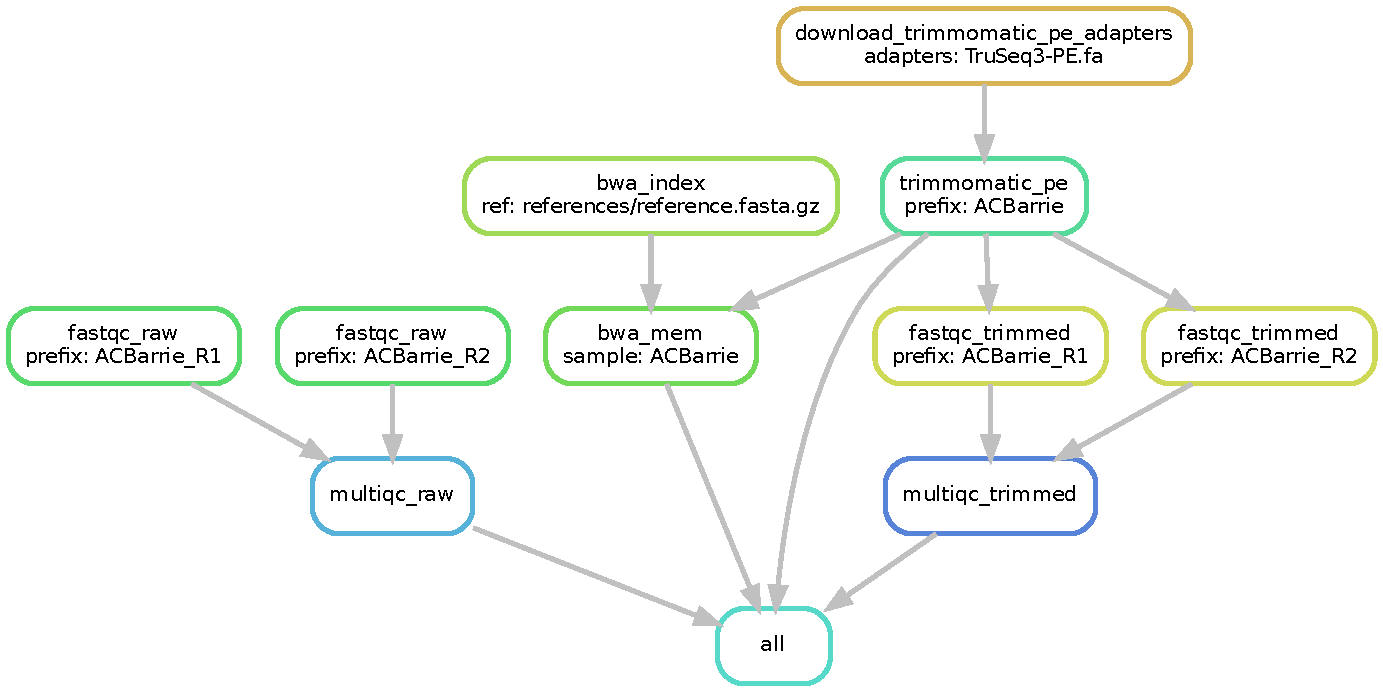
\includegraphics[width=0.8\textwidth]{handout/dag.pdf}
\caption{DAG of jobs where \texttt{accession} is \texttt{ACBarrie}.}
\label{fig:dag}
\end{figure}

The DAG's can get very large, very quickly. Uncomment the \texttt{Alsen} and \texttt{Baxter} lines in the \texttt{ACCESSIONS} list at the top of the
\texttt{Snakefile} and generate a new DAG. It will start to look like this:

\begin{figure}[H]
\centering
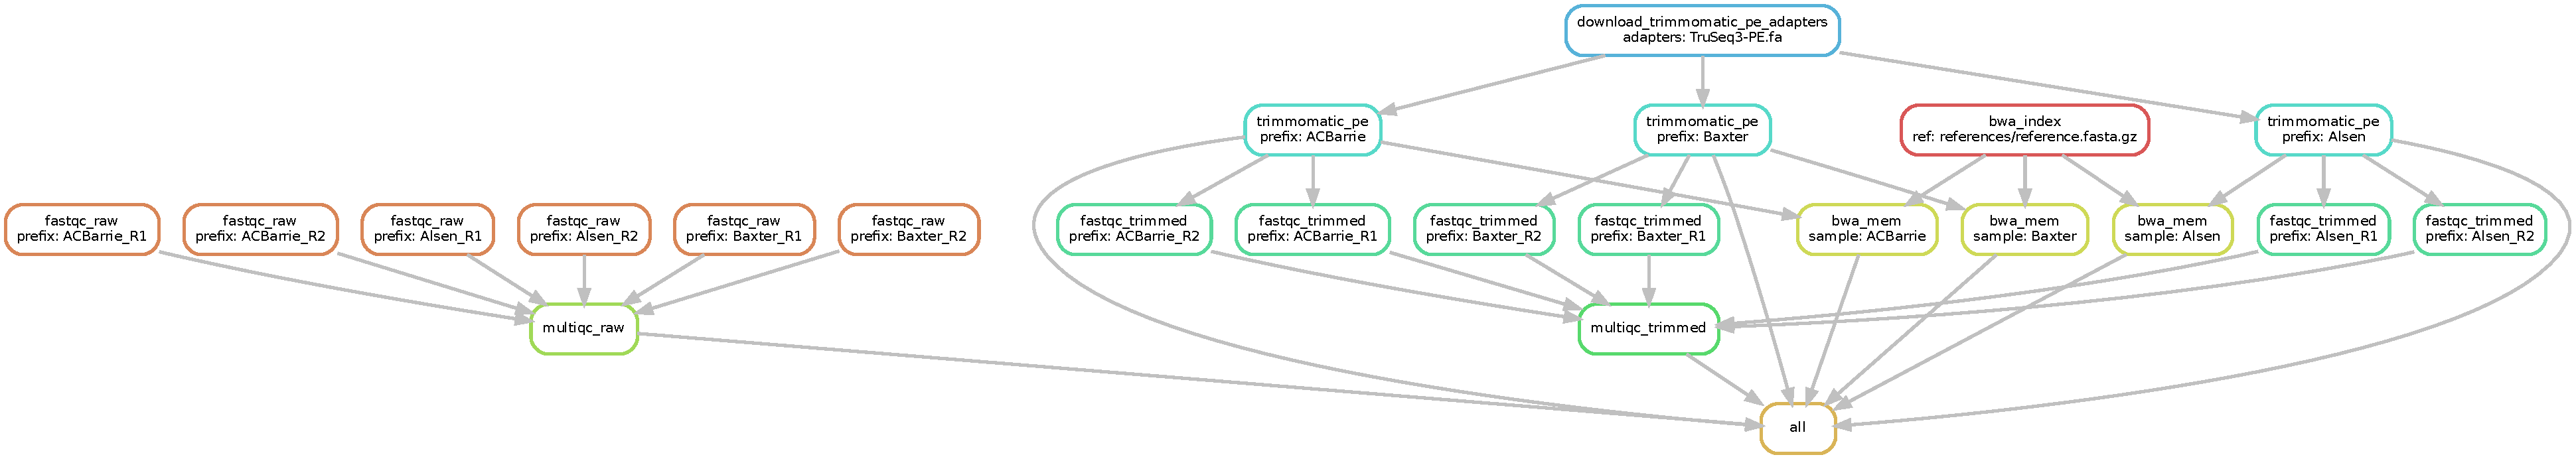
\includegraphics[width=0.8\textwidth]{handout/dag_bigger.pdf}
\caption{DAG of jobs where \texttt{accession} is \texttt{ACBarrie}, \texttt{Alsen} or \texttt{Baxter}.}
\label{fig:dag_bigger}
\end{figure}

Often it is enough to just look at the ``rulegraph'' which only contains information about the rules and the dependencies which exist between them:

\begin{lstlisting}
snakemake \
  --rulegraph \
| dot -Tpdf \
> rulegraph.pdf
\end{lstlisting}

\begin{figure}[H]
\centering
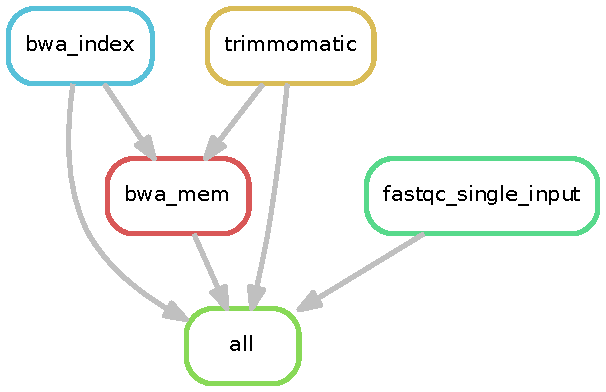
\includegraphics[width=0.8\textwidth]{handout/rulegraph.pdf}
\caption{Graph of rules.}
\label{fig:rulegraph}
\end{figure}

%------------------------
\subsection{Executing Jobs on an HPC Cluster}
%------------------------

So far we have been running snakemake on the cluster head node and any jobs it has been executing have also been on the head node. So far, this has been OK
since the jobs have been small and short-lived. However, individual jobs of a ``real-life'' bioinformatics workflow will have considerably larger resource
(CPU and RAM) requirements. If you continue executing these resource hungry jobs on the head node, your cluster sysadmin will start to growl at you!

Snakemake does not

Snakemake provides the ability to execute jobs within a singularity container and to have a conda software environment set up within it. This provides an opportunity

\begin{lstlisting}
module load \
  singularity-3.2.1-gcc-5.4.0-tn5ndnb

# Create the conda environment(s), ahead of running the workflow, by submitting a job to slurm
# This will take ~5mins
sbatch --job-name 'snakemake-env_setup' --mem 2G --time 30:00 --wrap \
  'snakemake --use-singularity --use-conda --create-envs-only'
\end{lstlisting}




%========================
\section{Modify/extend the Workflow}
%========================

%========================
\section{Your own Workflow}
%========================

%========================
\section{Snakemake Troubleshooting}
\label{sec:snake_trouble}
%========================

%------------------------
\subsection{Snakemake Install}
%------------------------

If you have a broken or incomplete snakemake installation, try the following steps to fix things:

\begin{lstlisting}
# deactivate the snakemake conda environment if it is already active
conda deactivate

# Delete the snakemake conda environment
conda env remove --name snakemake
\end{lstlisting}

Now try reinstalling snakemake.

%------------------------
\subsection{Conda Software Environment Setup}
%------------------------

If your job failed or timed out, you will need to re-run conda software environment setup job again. However, you may first need to release the
Snakemake lock which protects you from running multiple instances of the same workflow at the same time:

\begin{lstlisting}
snakemake \
  --unlock
\end{lstlisting}

To ensure Snakemake starts with a clean slate, delete the ``hidden'' \texttt{.snakemake} directory:

\begin{lstlisting}
rm -rf .snakemake
\end{lstlisting}

%------------------------
\subsection{Getting Going After a Disconnect}
%------------------------

If you find that your connection to the server has been dropped, you can get yourself going again using this convienient block of commands:

\begin{lstlisting}
# Load the required software modules
module load \
  miniconda3-4.6.14-gcc-5.4.0-kkzv7zk \
  singularity-3.2.1-gcc-5.4.0-tn5ndnb

# Activate the snakemake conda environment and integrate shell autocompletion into bash
conda activate snakemake
complete -o bashdefault -C snakemake-bash-completion snakemake

# Move to the correct directory location
cd /shared/${USER}/snakemake-tutorial
\end{lstlisting}
